% Quiz 07 --- Opinions on a network, and a knight on a chessboard. Printed, worked
% in class, 20 minutes, 10 points. Answers are photographed and uploaded to the
% Google Form (go.skojaku.com/ans-quiz07), one photo per question.
%
% Question 1 is the DeGroot model: every round, each person takes the average of
% their friends' opinions. The task is the final opinion. The lecturer walks
% through the model and the difference between the two ways to use P (a sender
% splits a probability; a receiver averages an opinion) before the quiz.
%
% Question 2 is a random walk of a chess knight on an 8 x 8 board.
%
% The answers are in solutions.tex.
%
% Compile with: xelatex -interaction=nonstopmode quiz07.tex   (run twice)
\documentclass[a4paper, 11pt]{extarticle}
% Shared preamble for Quiz 07 (quiz07.tex and solutions.tex).
% Compile with: xelatex -interaction=nonstopmode <file>.tex   (run twice)
%
% Same house look as the pen-and-paper sheets in
% lecture-note/*/pen-and-paper/: Charter, A4, generous leading, room to draw.

\usepackage[top=0.7in, bottom=0.6in, left=0.8in, right=0.8in]{geometry}
\usepackage{amsmath}
\usepackage{amssymb}
\usepackage{array}
\usepackage{graphicx}
\usepackage[hidelinks]{hyperref}
\usepackage{tcolorbox}
\usepackage{enumitem}
\usepackage{etoolbox}
\usepackage{tikz}
\usepackage{fontspec}
\usetikzlibrary{calc,positioning,arrows.meta}
\definecolor{pltblue}{HTML}{1F77B4}
\definecolor{rulegrey}{HTML}{6A6D75}

% Body face. Charter, and the four ways to get it. XCharter *is* Charter and
% ships with a full TeX Live, so it is asked for first and by file: a CI runner
% answers yes to \IfFontExistsTF{Charter}, then cannot typeset it.
\IfFontExistsTF{XCharter-Roman.otf}{
  \setmainfont{XCharter}[
    Extension      = .otf,
    UprightFont    = *-Roman,
    BoldFont       = *-Bold,
    ItalicFont     = *-Italic,
    BoldItalicFont = *-BoldItalic]
}{
  \IfFontExistsTF{Charter}{\setmainfont{Charter}}{
    \IfFontExistsTF{Iowan Old Style}{\setmainfont{Iowan Old Style}}{
      \IfFontExistsTF{Georgia}{\setmainfont{Georgia}}{}}}}

\setlength{\parindent}{0pt}
\setlength{\parskip}{0.4em}
\setlength{\emergencystretch}{1.2em}
\raggedbottom
\pagestyle{empty}

% ---------------------------------------------------------------------------
% The submission link.
%
% Both the QR square and the printed address are the course's own short link,
% not the form's: paper outlives any one form. Caddy on the course droplet
% points go.skojaku.com/ans-quiz07 at the current Google Form
% (/etc/caddy/Caddyfile, block go.skojaku.com). Swapping the form is a line on
% the server, not a reprint.
%
% If the link ever changes, rebuild the square with
%
%   uvx --from segno segno --output=quiz07-form-qr.png --scale=20 --border=1 \
%       --error=m "<the url>"
% ---------------------------------------------------------------------------
\newcommand{\formlink}{https://go.skojaku.com/ans-quiz07}
\newcommand{\formshort}{\href{\formlink}{\texttt{go.skojaku.com/ans-quiz07}}}

% Quiz header. #1 = title, #2 = the line under it, #3 = term.
\newcommand{\quizhead}[3]{%
  {\footnotesize\textsc{Advanced Network Science} \hfill \textsc{#3}}\par
  \vspace{-0.2em}\rule{\textwidth}{1pt}\par
  \vspace{0.3em}
  {\LARGE\bfseries #1}\par
  \vspace{0.1em}
  {\small #2}\par
  \vspace{0.7em}
  {\small Name \underline{\hspace{6cm}} \hfill Date \underline{\hspace{3.2cm}}}\par
  \vspace{0.7em}}

% A question heading with its point value.
\newcommand{\question}[3]{%
  \vspace{0.5em}
  {\large\bfseries Question #1 \quad\normalsize\mdseries (#2 points)}\par
  \vspace{-0.3em}{\color{rulegrey}\rule{\textwidth}{0.6pt}}\par
  \vspace{0.1em}
  {\bfseries #3}\par
  \vspace{0.2em}}

% An empty box to draw or write in. #1 = height, #2 = caption under the rule.
\newcommand{\drawbox}[2]{%
  \begin{tcolorbox}[colback=white, colframe=rulegrey, boxrule=0.5pt,
                    sharp corners, height=#1, valign=top,
                    boxsep=2pt, left=4pt, right=4pt, top=3pt, bottom=3pt]
  {\footnotesize\color{rulegrey} #2}
  \end{tcolorbox}}

% Ruled writing lines, #1 of them.
\newcommand{\writelines}[1]{%
  \vspace{0.3em}
  \foreach \i in {1,...,#1}{%
    {\color{rulegrey}\rule{\textwidth}{0.4pt}}\par\vspace{1.5em}}}


% Title and points share one line, as in Quiz 5 and 6.
\renewcommand{\question}[3]{%
  \vspace{0.4em}
  {\large\bfseries Question #1 \quad #3\quad\normalsize\mdseries (#2 points)}\par
  \vspace{-0.4em}{\color{rulegrey}\rule{\textwidth}{0.6pt}}\par}

\tikzset{
  gnode/.style={circle, draw=pltblue, fill=pltblue!12, line width=0.9pt,
                minimum size=6.5mm, inner sep=0pt, font=\small\bfseries},
  gedge/.style={line width=0.9pt, draw=rulegrey}
}

\begin{document}

\quizhead{Quiz 7 \; --- \; Opinions and a knight}
        {20 minutes \quad$\cdot$\quad 10 points \quad$\cdot$\quad
         Closed notes}
        {Fall 2026}

\begin{tcolorbox}[colback=white, colframe=rulegrey, boxrule=0.5pt,
                  sharp corners, boxsep=1pt, top=4pt, bottom=4pt]
\begin{minipage}[c]{0.14\textwidth}
\begin{center}

\includegraphics[width=1.6cm]{quiz07-form-qr.png}
\end{center}
\end{minipage}
\hfill
\begin{minipage}[c]{0.83\textwidth}
{\small
You hand in two photos, one per question. Write each question's answer on
its own page, photograph each page, and upload it. Point a camera at the
square, or type \formshort.
}
\end{minipage}
\end{tcolorbox}

% ---------------------------------------------------------------------------
\question{1}{6}{Opinions on a network.}

\begin{minipage}[c]{0.60\textwidth}
Five friends A--E are connected as drawn. Each holds an opinion on a proposal,
a number between 0 (against) and 1 (for). In every round, each person replaces
their opinion by the average of the opinions their friends held in the previous
round (friends only, not themselves). The opinions at the start are

\smallskip
\centerline{A $=0.8$,\; B $=0.2$,\; C $=0.6$,\; D $=0.4$,\; E $=1.0$.}
\end{minipage}
\hfill
\begin{minipage}[c]{0.37\textwidth}
\centering
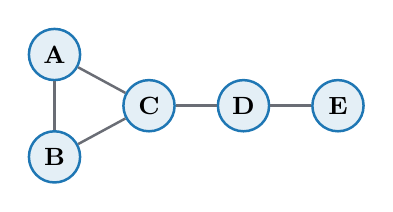
\begin{tikzpicture}[x=1.0cm, y=1.0cm]
  \node[gnode] (A) at (0.0, 0.9) {A};
  \node[gnode] (B) at (0.0,-0.4) {B};
  \node[gnode] (C) at (1.2, 0.25) {C};
  \node[gnode] (D) at (2.4, 0.25) {D};
  \node[gnode] (E) at (3.6, 0.25) {E};
  \foreach \a/\b in {A/B, A/C, B/C, C/D, D/E}
    \draw[gedge] (\a) -- (\b);
\end{tikzpicture}
\end{minipage}

\medskip
Let $x_i(t)$ be the opinion of person $i$ after $t$ rounds, $k_i$ the number of
friends of $i$, and $A_{ij}=1$ if $i$ and $j$ are friends and $0$ otherwise.
Then $x_i(t+1)=\sum_j P_{ij}\,x_j(t)$ with $P_{ij}=A_{ij}/k_i$. After many
rounds, everyone holds the same opinion $x^*$.

\medskip
(a) [1 pt] Compute the opinions after one round. Is the sum of the five opinions
the same as at the start?

\smallskip
(b) [2 pts] Find five numbers $w_A,\dots,w_E$, not all zero, for which
$\sum_i w_i\,x_i(t)$ is the same in every round. Show that your numbers work,
for any initial opinions.

\smallskip
(c) [1 pt] Find $x^*$.

\smallskip
(d) [2 pts] The eigenvalues of $P$ are $1,\ 0.654,\ -0.298,\ -0.500,\ -0.857$.
The gap between $x_i(t)$ and $x^*$ shrinks, round after round, roughly by a
fixed factor. Which of the five eigenvalues sets that factor, and what is it?
Explain in one or two sentences.

% ---------------------------------------------------------------------------
\question{2}{4}{A knight on a chessboard.}

A knight stands on an ordinary $8\times8$ chessboard. In every step it jumps to
one of the squares it can legally reach, each with the same probability. A jump
changes the column by 1 and the row by 2, or the column by 2 and the row by 1,
in either direction. Number the columns and the rows $1,\dots,8$. A square is
\emph{dark} if column $+$ row is even and \emph{light} otherwise (a1 is dark).
$P$ is the $64\times64$ transition matrix of the knight, and $p(t)$ is the
probability of each square after $t$ steps. The stationary distribution $\pi$
($\pi P=\pi$) puts probability $\tfrac12$ on the dark squares.

\medskip
(a) [1 pt] The knight starts at a1. What is the probability that it stands on a
dark square after $t$ steps, for $t=1,2,3,4$? Does $p(t)$ converge to $\pi$?

\smallskip
(b) [2 pts] Show that $-1$ is an eigenvalue of $P$. Name the eigenvector and
check it.

\smallskip
(c) [1 pt] Now the knight stays where it is with probability $\tfrac12$ and jumps
with probability $\tfrac12$. Its transition matrix is $\tfrac12(I+P)$. What
happens to the eigenvalue you found in (b)? Does $p(t)$ now converge to $\pi$?

\end{document}
